% Затехал Хасянов Расул
\section{Билет 17. Интегральное представление решений уравнений Лапласа и Пуассона в ограниченной области. Фундаментальное решение уравнения Лапласа.}
\subsection{Интегральное представление решений уравнений Лапласа и Пуассона в ограниченной области.}
Рассматривается уравнение Пуассона в $\R^3$: $\Delta u(x) = \brs{\pdd{}{x_1}+ \pdd{}{x_2}+\pdd{}{x_3}}u(x) = f(x), x \in \Omega \subset \R^3$, где $\Omega$ -- область.
\begin{definition}[Гармоническая функция]
Функция $u(x)$ называется гармонической в $\Omega \in R^3$, если \\ $u(x) \in C^2(\Omega)$ и $\Delta u(x) \equiv 0, \forall x \in \Omega.$ 
\end{definition}
Удобно перейти в сферическую систему координат: 
\[
\begin{cases}
x_1 = r \sin \theta \cos \varphi\\
x_2 = r \sin \theta \sin \varphi\\
x_3 = r \cos \theta.
\end{cases}
\]
Уравнение примет вид:
$$ 0 = \Delta \hat u (r, \theta, \varphi) = \hat u_{rr} + \frac{2}{r} \hat u_r + \frac{1}{r^2} \sbrs{\frac{1}{\sin \theta} \pd{}{\theta}\brs{\sin \theta \pd{\hat u}{\theta}}+ \frac{1}{\sin^2 \theta} \pdd{\hat u}{\varphi}}$$
В квадратных скобках написан оператор Лапласа-Бельтрани от функции $\hat u$.\\
Решение зависящее от $r$, удовлетворяет уравнению Эйлера: 
$$
\hat u_{rr}+ \frac{1}{r^2}\hat u_r = 0 \Rightarrow \hat u(r) = r^\mu \Rightarrow \mu(\mu-1) +2\mu =0 \Rightarrow \hat u(r) = C_1 + \frac{C_2}{r}$$
Функция $\hat u(r) = \frac{1}{r}$ -- гармоническая всюду кроме 0.
\begin{lemma}[Интегральное представление решения уравнения Пуассона]
Пусть $\Omega$ -- область с кусочно-гладкой границей $\Gamma$. Пусть $u(x) \in C^2(\Omega) \cap C^1(\bar \Omega), \Delta u \in C(\bar \Omega)$. Тогда для $\forall x \in \Omega\; u(x)$ представима в виде суммы трех потенциалов (объемного Ньютонова, простого слоя, двойного слоя): $$u(x) = \underbrace{\int_\Omega \brs{-\frac{1}{4\pi\abs{x-y}}}\Delta u(y) dy}_{\text{объёмный Ньютоновый потенциал}} - \underbrace{\oint_\Gamma \brs{-\frac{1}{4\pi\abs{x-y}}} \pd{u(y)}{\vec{n_y}}dS_y}_{\text{потенциал простого слоя}}+\underbrace{\oint_\Gamma \pd{}{\vec{n_y}}\brs{-\frac{1}{4\pi\abs{x-y}}}u(y)dS_y}_{\text{потенциал двойного слоя}}$$
\end{lemma}
\begin{proof}
Берем $x \in G, \varepsilon >0$ такое, что $\bar B(x,\varepsilon) \subset \Omega$ ($B$ -- открытый шар в $\R^3$). Строим область $\Omega_x^\varepsilon = \Omega \backslash \bar B(x, \varepsilon), \partial \Omega_x^\varepsilon = \Gamma \cup \gamma$, где $\gamma = \partial B(x,\varepsilon)$.\\
\begin{center}
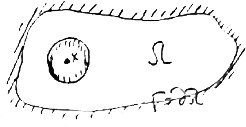
\includegraphics[width=0.2\textwidth]{17_1_new}
\end{center}
В $\Omega_x^\varepsilon$ ядро $K_3(x,y) = - \frac{1}{4\pi \abs{x-y}} \in C^\infty$ ($\Delta K_3(x,y) \equiv 0$). Используем 2 формулу Грина:
\begin{multline*}
\int_{\Omega_x^\varepsilon} \Delta u(y) K_3(x,y)dy - \int_{\Omega_x^\varepsilon} u(y) \Delta K_3(x,y)dy = {}\\
{}=\oint_\Gamma \pd{u(y)}{\vec{n_y}} K_3(x,y)dS_y + \oint_\gamma \pd{u(y)}{\vec{n_y}} K_3(x,y)dS_y - \oint_\Gamma u(y)\pd{}{\vec{n_y}} K_3(x,y) dS_y - \oint_\gamma u(y)\pd{}{\vec{n_y}} K_3(x,y) dS_y
\end{multline*}
\begin{multline*}
\Longleftrightarrow \int_{\Omega_x^\varepsilon} f(y) K_3(x,y)dy + \oint_\Gamma u(y)\pd{}{\vec{n_y}} K_3(x,y) dS_y - \oint_\Gamma \pd{u(y)}{\vec{n_y}} K_3(x,y)dS_y = {}\\
{} = \oint_\gamma \pd{u(y)}{\vec{n_y}} K_3(x,y)dS_y - \oint_\gamma u(y)\pd{}{\vec{n_y}} K_3(x,y) dS_y
\end{multline*}
\begin{offtop}
интеграл от $\frac{1}{\abs{x}^\alpha}$ сходится при $\alpha < n = \mathrm{dim}\, \R^n$. У нас $n=3, \alpha =1$.
\end{offtop}
Устремляем $\varepsilon \rightarrow 0$:
\begin{enumerate}
\item $\int_{\Omega_x^\varepsilon} \rightarrow \int_\Omega$ в силу последнего замечания.
\item
$
\oint_\gamma u(y) \pd{}{\vec{n_y}} \brs{-\frac{1}{4\pi} \cdot \frac{1}{|x-y|}}dS_y  = \frac{1}{4\pi \varepsilon^2} \oint \brs{u(y) - u(x) + u(x)}dS_y = \frac{1}{4\pi \varepsilon^2} \oint_\gamma \brs{u(y) - u(x)}dS_y + u(x)$\\
$\pd{}{\vec{n_y}} \brs{-\frac{1}{4\pi} \cdot \frac{1}{|x-y|}} \rightarrow \left.\frac{1}{4\pi}\brs{-\pd{}{\rho}\frac{1}{\rho}}\right|_{\rho = \varepsilon}$\\
$\frac{1}{4\pi \varepsilon^2} \abs{ \oint_\gamma \brs{u(y) - u(x)}dS_y} \leq \frac{1}{4\pi \varepsilon^2} \cdot \max\limits_{|y-x| \leq R} \abs{u(y)-u(x)} \cdot \oint_\gamma dS_y \rightarrow 0
$
\item
\begin{align*}
&\abs{\oint_\Gamma \pd{u(y)}{\vec{n_y}} K_3(x,y)dS_y} \leq \frac{1}{4\pi \varepsilon} M \int_\gamma dS_y = M \varepsilon \rightarrow 0\\
& \abs{\pd{u}{\vec{n_y}}} = \abs{(\nabla u, \vec n)} \leq \abs{\nabla u} \cdot \abs{n} \leq M, \text{ так как } \nabla u \in C\brs{\overline{\Omega}}
\end{align*}
\end{enumerate}
Итак, после предельного перехода получим требуемое соотношение
\end{proof}
\subsection{Фундаментальное решение уравнения Лапласа.}
Экскурс в обобщенные функции
\begin{definition}
$\mathcal{D}(\R^n)$ -- пространство пробных (основных) функций:\\ $\varphi(x) \in \mathcal{D}(\R^n) \Longleftrightarrow \varphi(x) \in C^\infty(\R^n),\; \mathrm{supp}\, \varphi(x)$ -- компакт. 
\end{definition}
\begin{definition}
В $\mathcal{D}(\R^n)$ вводится сходимость по следующему правилу: $\fbrs{\varphi_k(x)}_{k=1}^{\infty} \rightarrow \varphi(x) \in \mathcal{D}(\R^n) \Longleftrightarrow$
\begin{itemize}
\item $\forall \alpha = (\alpha_1, \ldots, \alpha_n)\; \mathcal{D}^\alpha \varphi_k \rightrightarrows \mathcal{D}^\alpha \varphi$
\item $\exists A > 0: \varphi_k (x) \equiv 0$ при $|x| > A, \forall k \in \N$ (у всех функций общий носитель)
\end{itemize}
\end{definition}
Пример функции из $\mathcal{D}(\R^n)$: 
$$\omega_\varepsilon(x) = \begin{cases}\frac{1}{\varepsilon^n}e^{-\frac{1}{1-\brs{x/\varepsilon}^2}}, |x| \leq \varepsilon \\ 0, |x| > \varepsilon \end{cases} \Rightarrow \mathcal{D}(\R^n) \neq \varnothing$$
\begin{definition}
Обобщенная функция $f$ над $\mathcal{D}(\R^n)$ -- всякий линейный непрерывный функционал над $\mathcal{D}(\R^n)$
\end{definition}
\begin{definition}
Линейный функционал: $(f, \alpha \varphi + \mu \psi) = \alpha (f, \varphi) + \mu (f, \psi)$
\end{definition}
\begin{definition}
Непрерывный функционал: $\forall \fbrs{\varphi_k} \rightarrow \varphi$ в  $\mathcal{D}(\R^n) \Rightarrow f(\varphi_k)\rightarrow f(\varphi)$
\end{definition}
По определению $\forall \lambda, \mu \text{ -чисел}, \forall f, g \in \mathcal{D}'(\R^n)$ обобщенная функция $F = \lambda f + \mu g \in \mathcal{D}'(\R^n), \;\\(F, \varphi)  \stackrel{\mathrm{def}}{=} \lambda (f, \varphi) + \mu (g, \varphi)$
\begin{definition}[сходимость в $\mathcal{D}'(\R^n)$]
$\fbrs{f_n}_{n=1}^\infty \rightarrow f \in \mathcal{D}'(\R^n) \stackrel{\mathrm{def}} {\Longleftrightarrow} (f_k, \varphi) \rightarrow (f, \varphi), \forall \varphi \in \mathcal{D}(\R^n)$ (слабая$^*$ сходимость). 
\end{definition}
\begin{definition}
Функция $f(x)$ называется локально интегрируемой, если $\forall B > 0\; \exists \int_{|x| < B} \abs{f(x)}dx < \infty$. 
\end{definition}
Каждая такая $f(x)$ порождает обобщенную функцию $(f,\varphi) = \int_{\R^n} f(x) \varphi(x) dx$.\\
Если существует локально интегрируемая $f(x)$ такая, что обобщенная функция $f$ представляется в виде $(f,\varphi) = \int_{\R^n} f(x) \varphi(x) dx$, то $f \in \mathcal{D}'(\R^n) $ называется регулярной.
\begin{lemma}[Дюбуа-Реймон]
Если $f$ и $g$ непрерывны и порождают одну обобщенную функцию, то $f \equiv g$. Если $f$ и $g$ разрывны, то они совпадают почти всюду.
\end{lemma}
\begin{definition}[$\delta$-функция]
$(\delta, \varphi) \stackrel{\mathrm{def}}{=} \varphi(0)$
\end{definition}
$\delta$-функция не является регулярной. \\
Обобщенные функции бесконечно дифференцируемы.\\
Правило дифференцирования: $(\mathcal{D}^\alpha f, \varphi) = (-1)^{|\alpha|} (f, \mathcal{D}^\alpha \varphi)$.\\
В частном случае $(\Delta f, \varphi) = (f, \Delta \varphi)$
\begin{theorem}
Функция $E(x) = \frac{-1}{4\pi |x|}$ является решением в обобщенных функциях уравнения $\Delta E(x) = \delta(x)$.
\end{theorem}
\begin{proof}
Пусть $\varphi \in \mathcal{D}(\R^n), \mathrm{supp} \varphi \subset B(0, A)$. Возьмем $\Omega = B(0, A +1)$. По теореме об интегральном представлении
\begin{align*}
\varphi(0) &= \int_{|y| < A +1} E(y) \Delta_y \varphi(y) dy + \cancel{\oint_{|y| = A+1} \varphi(y)\pd{E(y)}{\vec{n_y}} dS_y} - \cancel{\oint_{|y| = A+1} \pd{\varphi(y)}{\vec{n_y}} E(y)dS_y} = \\
&= (E, \Delta_x \varphi(x)) = (\Delta E, \varphi(x))
\end{align*}
Что и требовалось.
\end{proof}
\begin{definition}
Функция $E(x)$ называется фундаментальным решением оператора Лапласа.
\end{definition}